\documentclass[12pt,t]{beamer}
\usetheme[style=simple,nat,en]{Frederiksberg}
\usepackage{pslatex}
\usepackage[utf8]{inputenc}
\usepackage{color}
\usepackage{graphicx}
\usepackage{pgf}
\usepackage{pgfplots}
\usepackage{tikz}
\usetikzlibrary{arrows,automata,fit}
\usepackage{listings}% http://ctan.org/pkg/listings
\lstset{
      basicstyle=\ttfamily,
        mathescape
    }

\title{Scalable backend for Online TA}
\subtitle{}
\author{Simon Maibom \& René Løwe Jacobsen}
\institute{Department of Computer Science}
\begin{document}
\frame[plain]{\titlepage}
\begin{frame}
\frametitle{Introduction}
\begin{itemize}
    \item Distributed system
    \item Support multiple sandbox types
    \item Prevent plagiarism charges
\end{itemize}
\end{frame}
\begin{frame}
\frametitle{Architecture and analysis}
\begin{itemize}
    \item Master - node
    \item Dynamic adding and removal of nodes
    \item Distribution of submissions
    \item Handling of node failure
\end{itemize}
\includegraphics[scale=0.3]{design.png}
\end{frame}
\begin{frame}
\frametitle{Security}
\begin{itemize}
    \item Trusted modules
    \item Authorization and authentication
    \item Single point of failure
\end{itemize}
\end{frame}
\begin{frame}
\frametitle{Results}
    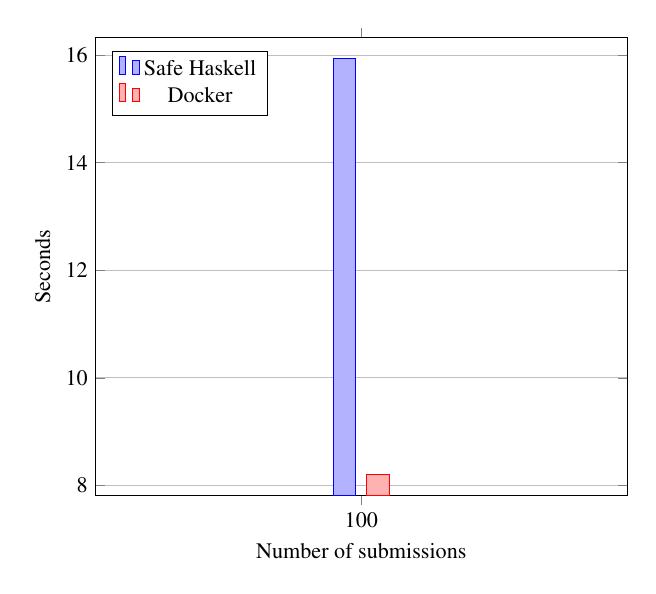
\begin{tikzpicture}[scale = 0.8]
        \begin{axis}[
            ymajorgrids=true,
            ylabel=Seconds,
            xlabel=Number of submissions,
            xtick=data,
            enlargelimits=0.05,
            % symbolic x coords={SafeHaskell,Docker},
            legend style={at={(0.03,0.97)},anchor=north west},
            ybar=5pt,% configures `bar shift'
            scale only axis
        ]
            % Original
            \addplot coordinates {(100,15.94)};
            % Optimized
            % 1 dimensional
            \addplot coordinates {(100,8.2)};
            % i32 implementation
            %\addplot coordinates {(Small,16299.30)};
            % f32 implementation
            %\addplot coordinates {(Small,18656.20)};
            % Parboil
            %\addplot coordinates {(Small,8031.67)};

            \legend{
                Safe Haskell,
                Docker
                %1 dimensional,
                %i32 implementation,
                %f32 implementation,
                %Parboil
                }
        \end{axis}
    \end{tikzpicture}
\end{frame}

\begin{frame}
\frametitle{Results}
    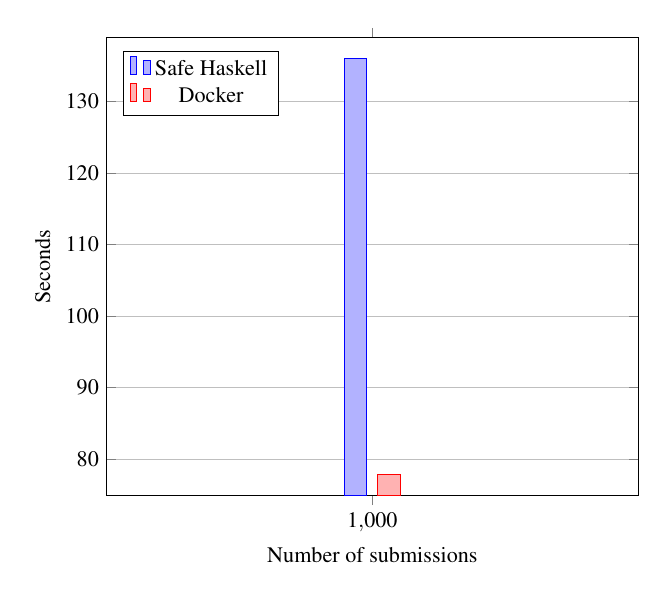
\begin{tikzpicture}[scale = 0.8]
        \begin{axis}[
            ymajorgrids=true,
            ylabel=Seconds,
            xlabel=Number of submissions,
            xtick=data,
            enlargelimits=0.05,
            % symbolic x coords={SafeHaskell,Docker},
            legend style={at={(0.03,0.97)},anchor=north west},
            ybar=5pt,% configures `bar shift'
            scale only axis
        ]
            % Original
            \addplot coordinates {(1000,136.08)};
            % Optimized
            % 1 dimensional
            \addplot coordinates {(1000,77.82)};
            % i32 implementation
            %\addplot coordinates {(Small,16299.30)};
            % f32 implementation
            %\addplot coordinates {(Small,18656.20)};
            % Parboil
            %\addplot coordinates {(Small,8031.67)};

            \legend{
                Safe Haskell,
                Docker
                %1 dimensional,
                %i32 implementation,
                %f32 implementation,
                %Parboil
                }
        \end{axis}
    \end{tikzpicture}
\end{frame}
\begin{frame}
\frametitle{Conclusion and future works}
\begin{itemize}
    \item Large project scope, maybe to large?
    \item Working prototype
    \item A webinterface and auth
\end{itemize}
\end{frame}
\end{document}

1000 haskell - 2:16,08
100 haskell - 15,94

1000 docker - 1:17,82
100 docker - 8,2